\scanpage{79}
\uline{Corollaire} 1 $V$ anneau de val. discrète \inserted{hensélien, corps résiduel $\unsure{k}$,} $K$ corps des fractions, \inserted{$\overline K$ clôture alg.,} $A$ schéma abélien sur $K$, $G$ modèle de Néron de $A$, \inserted{$T$ tore maximal de $G_k$,} \deleted{$\unsure{G}\text{ de }T_\ell(A)\unsure{\to|\supset}$} $\ell$ nb premier $\ne\operatorname{car}.k$, \deleted{\unsure{$0\longrightarrow$|On a} $\widetilde{T_\ell(G_k)}|U$} donc
\[
\widetilde{T_\ell(\deleted{\unsure{G|C}}\inserted{T})}|U\subset\widetilde{T_\ell(G_k)}|U\subset T_\ell(\unsure{A'|A})
\]
et en prenant les points à valeurs dans $\overline K$
\[
M(\deleted{\unsure{T}}\inserted{A})_0^I\subset M(\deleted{\unsure{G_k|G|T}}\inserted{A})^I\subset M(A)=T_\ell(A(\overline K))\deleted{=T_\ell(A)(\overline K)}
\]
où $I$ est le groupe d'inertie $\subset\pi=\operatorname{Gal}(\overline K/K)$, et où l'exposant $I$ désigne les invariants sous $I$.
Ceci posé, si $A'$ est une deuxième variété abélienne \inserted{\uline{sur} $\unsure{k|K}$.} et $\xi$ une \deleted{\unsure{donnée de}} corr. divisorielle sur $A\times A'$, d'où un accouplement compatible avec $\pi$ donc $I$
\[
\varphi_\xi:M(A)\times M(A')\mathbin{-}T_\ell(\overline K^*)\deleted{=T_\ell(\mathbf G_m\unsure{)}},
\]
on a : \deleted{\unsure{les|la} \unsure{relations|relation}} $M(A)^I$ et $M(A')_0^I$ sont ortho-
gonaux, ainsi que $M(A)_0^I$ et $M(A')^I$.

En particulier

\uline{Corollaire 2} Soit $\xi$ une \uline{polarisation} sur $A$, d'où
\margin{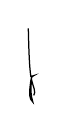
\begin{tikzpicture}[x=0.12cm,y=0.12cm]\draw[line width=0.45pt] (0,8) .. controls (0.05,6) and (0.10,4) .. (0.27,2.9) -- (0.60,3.0) .. controls (0.30,2.95) and (0.27,2.5) .. (0.22,2.1) .. controls (0.09,1.1) and (0.09,0.5) .. (0.48,0.2) .. controls (0.28,0.8) and (0.20,1.6) .. (0.36,2.5) .. controls (0.48,1.9) and (0.85,1.25) .. (0.58,0.9);\end{tikzpicture}}
une forme bil. alternée non dégénérée sur
\[
\varphi_\xi:M(A)\times M(A)\unsure{\mathbin{-}|\longrightarrow}T_\ell(\overline K^*)
\]
Alors
\[
\varphi_\xi(M^I,M_0^I)=0.
\]
En fait, les deux corollaires sont à priori équivalents, comme on constate aisément $\ldots\ldots$

\uline{Remarque} A la limite projective, \inserted{si $k$ est sép. clos,} les \unsure{hom|homo}
\[
\unsure{\alpha|\text{en}|\deleted{\ell^\nu}}\qquad {}_{\unsure{\ell^\nu}}A'(K)\times{}_{\ell^\nu}T(k)\to{}_{\ell^\nu}k^*\simeq{}_{\ell^\nu}K^*
\]
sont nuls. Cependant ces \unsure{accouplts|accouplements} eux mêmes ne
\margin{78}
